\documentclass{article}
\usepackage[english]{babel}
\usepackage[utf8]{inputenc}
\usepackage{subcaption}
% for mathematics
\usepackage{amsmath}
\usepackage{amsthm}
% define theorems, lemmas, etc
\newtheorem{theorem}{Theorem}
\newtheorem{lemma}{Lemma}
\newtheorem{corollary}{Corollary}
\newtheorem{definition}{Definition}
\newtheorem{example}{Example}
\usepackage{amssymb}

% for adjusting margins
\usepackage{geometry}
\geometry{
	a4paper,
 	left=26mm,
 	right=20mm,
 	top=33mm,
 	bottom=38mm
}

% for coding import
\usepackage{listings}
\usepackage{color}
\usepackage{csquotes}

\definecolor{codegreen}{rgb}{0,0.6,0}
\definecolor{codegray}{rgb}{0.5,0.5,0.5}
\definecolor{codepurple}{rgb}{0.58,0,0.82}
\definecolor{backcolour}{rgb}{0.95,0.95,0.92}
 
\lstdefinestyle{mystyle}{
    backgroundcolor=\color{backcolour},   
    commentstyle=\color{codegreen},
    keywordstyle=\color{magenta},
    numberstyle=\tiny\color{codegray},
    stringstyle=\color{codepurple},
    basicstyle=\footnotesize,
    breakatwhitespace=false,         
    breaklines=true,                 
    captionpos=b,                    
    keepspaces=true,                 
    numbers=left,                    
    numbersep=5pt,                  
    showspaces=false,                
    showstringspaces=false,
    showtabs=false,                  
    tabsize=2
}
\lstset{style=mystyle}

% for introducing urls
\usepackage{url}

% for colored text
\usepackage{color}

% for creating lists
\usepackage{enumerate}

% for import graphics
\usepackage{graphicx}
\setcounter{secnumdepth}{5}
\usepackage{floatrow}

%\usepackage{times}
% we opt not to use the times new roman font family

% title details
\title{CS3244 Machine Learning Homework 3 Report}
\author{Kaggle Group HEHEDA: A0148008J, A0141132B}


\begin{document}


% insert title
\maketitle



\begin{abstract}
This document is the README file our group submit for the detailed report for homework3 of CS3244 Machine Learning. In this homework, we chose the first task which is to predict the sales of many stores and try to minimise the defined prediction error function. We divide the following README into three main sections: preliminary analysis, initial attempt and improving the prediction. We have included some supporting figures in the appendix. The extra help we sought from other online resources will be acknowledged in the references list.\\

The following is a list of our submission files.\\

  \begin{enumerate}
  \item \textbf{hw3-rossman.ipynb} : source code and our core answers. It contains the full code of our model implementation and it has been divided into sections. Every output can be reproduced by running that cell given the previous all cells have been run before.
  \item \textbf{README.pdf} : report of our homework, the current file you are reading. It contains all the necessary thinking and model developing process. The full rationale and collated output can be found in this document.
  \end{enumerate}
  
\end{abstract}

\newpage

\tableofcontents

\newpage

\newpage

\section{Preliminary Analysis}
As we want to learn from data, we firstly conducted a preliminary analysis on the data we have, which are the $store.csv$ and the $train_{v2}.csv$ file. We used python to conduct this data research and got the following discoveries about the data.
\subsection{Feature Analysis}
\textbf{Store}: There are totally 1115 stores.\\
\textbf{StoreType}: Differentiates between 4 different store models: a, b, c, d.\\
\textbf{Assortment}: Describes an assortment level: a = basic, b = extra, c = extended.\\
\textbf{CompetitionDistance}: There are some stores without competitions nearby. The minimum competition distance is 20 and the longest distance is 75860.\\
\textbf{PromoInterval}: There are three types of promotion intervals, given by this list: ['Jan,Apr,Jul,Oct', 'Feb,May,Aug,Nov', 'Mar,Jun,Sept,Dec']\\
\textbf{Open}: If the store is closed on that day, the sales will be zero. We will assume this when processing the testing data.\\
\textbf{Sales}: If the sales of the store on that day is zero, then the store is closed on that day. We will assume this when processing the testing data.\\
\textbf{StateHoliday}: On state holiday, the store might not be closed.\\
\textbf{SchoolHoliday}: On state holiday, that day might not be school holiday.
\subsection{Modelling Analysis}
\subsubsection{Combined prediction with different stores}
In this problem, we can see there are over 1000 stores' sales to predict. The stores have quite a lot features, and most of them differ from each other. Although one can argue that different stores should have different model also because of their intrinsic differences including quantitative difference such as local population, and the qualitative inconsistencies like the service quality and reputation of specific stores, we decided to combine the prediction model for all stores together as there are not enough data points for each store. The stores are similar enough that they can be considered together. We will also add store specific values into each row of training data to signal different stores and their differences.
\subsubsection{Special treatment for time series data}
As we can see from the training data, the data given (store's sales) is a type of time series data. Time series data has a order, thus making it completely different from normal machine learning data and some special treatments should be applied. In this case, we firstly plotted all the necessary graphs about training data using  Excel aiming to have a clearer grasp of it.\\

\begin{figure}[h]
	\centering
	\includegraphics[scale=0.35]{validation_time_series.png}
	\caption{Method we use to do cross validation for time series data}
\end{figure}

This method could be unused if we utilise the xgboost library's own cross validation function.


\subsubsection{Plots and discoveries}
We have plotted several graphs after getting the raw data from the csv files. Part of the code has been given inside the notebook $preliminary analysis.ipynb$. More plots with rationale for feature selections are listed in the appendices.\\
We firstly plotted the stores' sales time series data, using time as the x-axis, and the sales figure as the y-axis.\\
\begin{figure}[h]
	\centering
	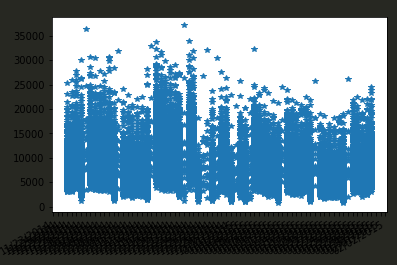
\includegraphics[scale=0.35]{sales_time_series.png}
	\caption{Sales time series data excluding store close dates}
\end{figure}

we can see from this figure that the sales of different stores among different dates are roughly between 2500 to 20000. There's so clear relation between the sales figures and the dates. In addition, there are clusters (different stores clustered together), which may demonstrate the time effect in the sales prediction.

\begin{figure}[h]
	\centering
	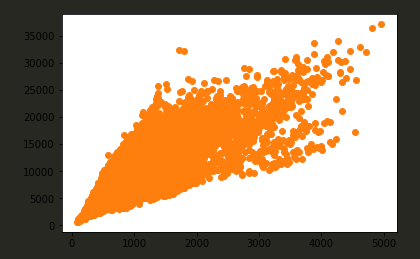
\includegraphics[scale=0.35]{customer_sales.png}
	\caption{Sales and number of customers}
\end{figure}

In this figure, we see clear correlation between the number of customers and the sales figure, which means if we have more customers in a particular day, we should expect more sales. Number of customers should be surely included inside the model.

\begin{figure}[h]
	\centering
	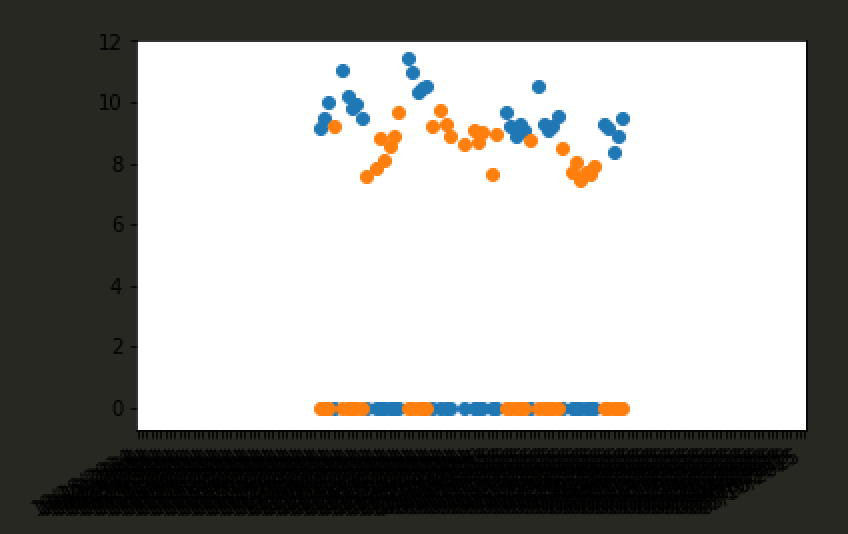
\includegraphics[scale=0.35]{typical_promotion_effect.png}
	\caption{Sales figure with promotion (blue) versus without promotion (orange) for a particular store}
\end{figure}

Next, from this plot, clearly for a single store, the sales figures will be slightly higher. The promotion factor should also play a very important role in the model.

\newpage

\section{Initial attempt}


\subsection{Choosing the model}
Taking into account of the fact that there are some test cases, whose features we don't know, we cannot guarantee the correctness and the feasibility of using a time series data modelling. By extensive online research, we decided to use extreme gradient boosting model to conduct the regression and prediction as a first try.

\subsection{Data Modelling}
We chose to do the following features as the full model. The features include: current day of week, number of customers, today's promotion state (boolean), today's state holiday and school holiday state, whether the current month is in promotion period, the store type, the store's assortment, the day count since the promotion starts and the store's promotion interval.\\

We $firstly$ remove the not open stores' row in both training and testing data, we will recover those zero rows in the end as we are sure that those not opening stores will have zero sales. $Secondly$, the feature of competition each store is having is calculated as a reciprocal of current competition, so that if there's no information about that store's competition, we can assign zero competition to that store, meaning the competition distance is infinity and there's no competition nearby.\\

From online discussion, some of the original wining teams have done logged sales as an alternative label column, so we split the training set into features column and the label (sales) column and took the logarithm of the sales to be our second model. Now we have two full models, namely the $full Model$ and the $log Model$.\\

For stores, we have utilized the training data set to get some specific information about each store, including the average sales, average sales per customers and the average open ratio, $etc$. These are calculated based on logged sales for the $log Model$ Following that, we conducted a natural join of store information and the training entries by using store index number.\\

After splitting the sales column out of the training entries, we performed categorical data conversion. Because of the nature of the model (extreme gradient boosting), we cannot feed the model with categorical (string type) data, which cannot be converted into floating number. When dealing with categorical variables, we have several approaches, including numeric encoding, binary encoding and one hot encoding. Below shown is a graph demonstrating the relative accuracy among different categorical data modelling methods.

\begin{figure}[h]
	\centering
	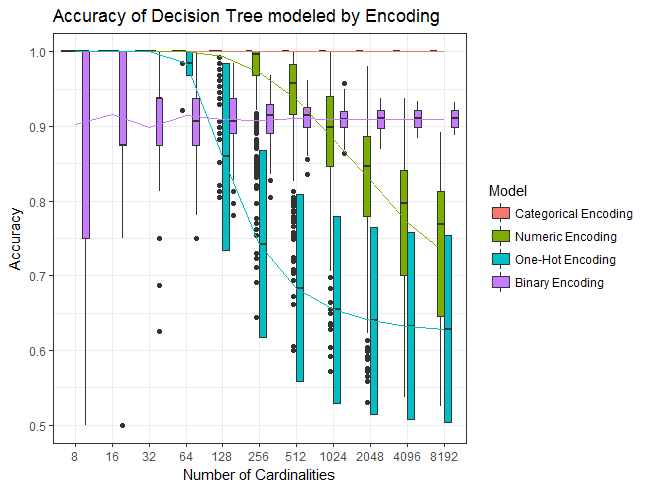
\includegraphics[scale=0.30]{categorical_encoding.png}
	\caption{Comparison between categorical encoding methods}
\end{figure}

Considering the relatively small cardinality and the feature number we have gotten, we decided to perform one hot encoding, which requires us to encode the training set and the testing set together to eliminate the corner case that the testing set has some new categories for some features column.

\subsection{Implementation and results}
Without customizing the objective function and any validation, we directly perform extreme gradient boosting using $XGBoost$ python package with default parameters. Although the kaggle score we get from this round is $0.36471$, we aims to perform validation to get a better estimate of our $E_{out}$. In the following section, we will try to improve our prediction with different Machine learning models, different data modelling, different feature selections and cross validation techniques.

\begin{center}
 \begin{tabular}{||c c c c c c c||} 
 \hline
 Model Name & 1st CV & 2nd CV & 3rd CV & 4th CV & 5th CV & Average CV Error \\ [0.5ex] 
 \hline\hline
 Full Model & 0.108 & 0.157 & 0.163 & 0.125 & 0.088 & 0.128 \\ 
 \hline
 Logged Model & 0.131 & 0.156 & 0.086 & 0.081 & 0.072 & 0.105 \\ [1ex] 
 \hline
\end{tabular}
\end{center}


\section{Improving the prediction}
\subsection{Validation}
\subsubsection{One step validation}
We $Firstly$ applied one step validation using the newest 6000 data entries as the validation set. Using this validation technique, we tuned some of our parameters of the gradient boosting to try to achieve a smaller validation error. $Next$, we tried to plot the relative importance of our model and try to select a few that are good to have and actually improving our out sample estimation. 

\begin{figure}[h]
	\centering
	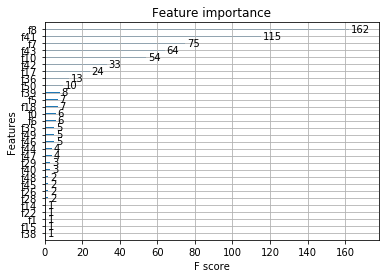
\includegraphics[scale=0.5]{comparison_between_features.png}
	\caption{Comparison of importance between our initial set of features}
\end{figure}

From the plot, we can see some of our features are very important, and some of them can be removed to prevent over fitting, we have prepared our current data modelling's header so that we can select features based on this importance plot.

\subsubsection{Cross validation}
For the ease of feature selection, model selection and parameter tuning, we wrote a cross validation function using the implementation as we have previously discussed for time series data. This function is able to do k fold cross validation without massing up the order of the training data entries to make it always validating the later time data. Each round, we will calculate the validation error. In the end, we will also have the average validation error as a better estimate. In each round of model selection, we also tuned the parameters of the models and tried to minimise the cross validation based on the best parameters set.
 
\subsection{Data Modelling}
As in the testing data, we already have the customer number, it is natural to consider the sales customer ratio as the new label, and we name this model as $ratioModel$. For our prediction and error calculation, we must use the final prediction figure. Therefore, we wrote some helper functions to restore the sales prediction from the predicted ratios, to restore the sales prediction from the logged prediction, and to restore the zero values from the closed stores to make our prediction ready for final submission.

\begin{center}
 \begin{tabular}{||c c c c c c c||} 
 \hline
 Model Name & 1st CV & 2nd CV & 3rd CV & 4th CV & 5th CV & Average CV Error \\ [0.5ex] 
 \hline\hline
 Ratio Model & 0.072 & 0.077 & 0.081 & 0.091 & 0.062 & 0.076 \\[1ex] 
 \hline
\end{tabular}
\end{center}

\subsection{Feature selection}
From the testing dataset, and the training data set, we found the difference between the dates. There is no difference in year and no overlap in month. That is to say, month and year is not needed for our prediction purposes. Except the number of customers, we also calculated average sales for different stores with and without promotion. When Joining the stores and training entries, we will join the store with its no promotion average sales figure if the store was not on promotion on that day. Similarly, we added variance, median, and sales customer ratios.\\

Thanks to the XGBoost library's built-in feature selection functions, we can plot the relative importance of each feature, and try to select a subset of our original features based on that to prevent over fitting. Therefore, we wrote two helper functions to get the important features using self-defined importance threshold and select the feature columns for training based on the selected feature indices. After validation across some subsets of features we chose and cross validation, we have the following results. As we find out, selecting a subset of the full model's features doesn't improve much on the cross validation error. Consequently, we used full features to implement the ensemble methods in the following section.\\

In these partial models, the following features typically show higher importance over the others from selected index: \textit{Average sales customer number Ratio, Day of week, Number of Customers, School Holiday, Month In Promotion, promotion Interval, Average Sales, competition Day Count, Variance SC Ratio, promotion Day Count, Sales Variance.}

\begin{center}
 \begin{tabular}{||c c c c c c c||} 
 \hline
 Model Name & 1st CV & 2nd CV & 3rd CV & 4th CV & 5th CV & Average CV Error \\ [0.5ex] 
 \hline\hline
 Partial Full Model & 0.109 & 0.174 & 0.094 & 0.092 & 0.068 & 0.107 \\ 
 \hline
 Partial Logged Model & 0.123 & 0.153 & 0.078 & 0.078 & 0.078 & 0.102 \\ 
 \hline
 Partial Ratio Model & 0.074 & 0.070 & 0.075 & 0.092 & 0.062 & 0.075 \\ [1ex] 
 \hline
\end{tabular}
\end{center}


\subsection{Ensemble regression method}
A first attempt was to combine the two available xgboost model's linear and tree methods. We have tried using harmonic mean and simple average. In addition, we chose to use SKLearn's ensemble regression model, we used regressors from adaptive boosting, bagging, extra tree model, gradient boosting and random forest. There's a small improvement when using bagging regressor, the results are collated in the following table. As we can see, the cross validation performance is very similar to the XGBoost model.\\

\begin{center}
 \begin{tabular}{||c c c c c c c||} 
 \hline
 Model Name & 1st CV & 2nd CV & 3rd CV & 4th CV & 5th CV & Average CV Error \\ [0.5ex] 
 \hline\hline
 AdaBoost Full Model & 0.212 & 0.453 & 0.295 & 0.291 & 0.262 & 0.302 \\ 
 \hline
 AdaBoost Logged Model & 0.165 & 0.350 & 0.190 & 0.205 & 0.173 & 0.217 \\ 
 \hline
 AdaBoost Ratio Model & 0.086 & 0.083 & 0.095 & 0.119 & 0.090 & 0.095 \\ 
 \hline
  Bagging Full Model & 0.096 & 0.161 & 0.090 & 0.097 & 0.066 & 0.102 \\ 
 \hline
  Bagging Logged Model & 0.096 & 0.172 & 0.082 & 0.093 & 0.066 & 0.102 \\ 
 \hline
  Bagging Ratio Model & 0.074 & 0.084 & 0.087 & 0.086 & 0.061 & 0.078 \\ 
 \hline
  Extra Tree Full Model & 0.135 & 0.207 & 0.130 & 0.103 & 0.071 & 0.129 \\ 
 \hline
  Extra Tree Logged Model & 0.123 & 0.202 & 0.129 & 0.098 & 0.070 & 0.125 \\ 
 \hline
  Extra Tree Ratio Model & 0.077 & 0.090 & 0.091 & 0.088 & 0.072 & 0.084 \\ 
 \hline
   Gradient Boosting Full Model & 0.120 & 0.174 & 0.122 & 0.126 & 0.081 & 0.125 \\ 
 \hline
   Gradient Boosting Logged Model & 0.011 & 0.151 & 0.103 & 0.105 & 0.070 & 0.108 \\ 
 \hline
   Gradient Boosting Ratio Model & 0.073 & 0.073 & 0.083 & 0.097 & 0.061 & 0.077 \\ 
 \hline
   Random Forest Full Model & 0.098 & 0.161 & 0.085 & 0.096 & 0.065 & 0.101 \\ 
 \hline
   Random Forest Logged Model & 0.095 & 0.173 & 0.080 & 0.092 & 0.065 & 0.101 \\ 
 \hline
   Random Forest Ratio Model & 0.074 & 0.083 & 0.087 & 0.086 & 0.060 & 0.078 \\ [1ex] 
 \hline
\end{tabular}
\end{center}


\subsection{Model shortlisting and final prediction}
As there are intrinsic assumptions behind each model, and some of these assumption can slightly affect the prediction, we have shortlisted the following models' predictions as they generally have lower cross validation error (smaller than 0.12 as our threshold) and they are consistent in sample predictions:\\\\
$Ratio Model$, $Partial Ratio Model$, $Logged Model$, $Partial Full Model$, $Partial Logged Model$, $adaBoost Ratio Model$, $Bagging Full Model$, $Bagging Logged Model$, $Bagging Ratio Model$, $Extra Tree Ratio Model$, \\$Gradient Boosting Logged Model$, $Gradient Boosting Ratio Model$, $Random Forest Full Model$, \\$Random Forest Logged Model$, $Random Forest Ratio Model$\\\\
Averaging arithmetically all of the above model's prediction, we get our final prediction.





\newpage
\section{Appendix}
\subsection{Other notable plots for feature selections}
\begin{figure}[h]
	\centering
	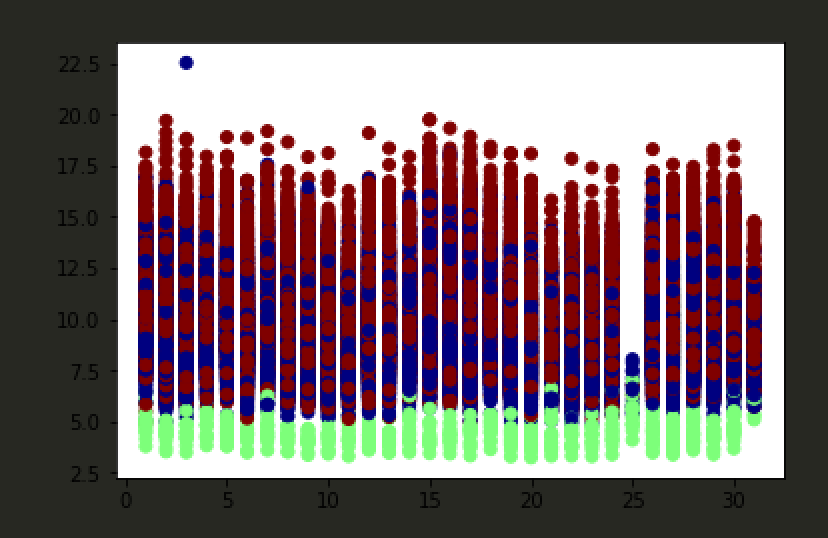
\includegraphics[scale=0.3]{Features/assortment.png}
	\caption{Different Sales Customer ratio against store assortment}
\end{figure}
\begin{figure}[h]
	\centering
	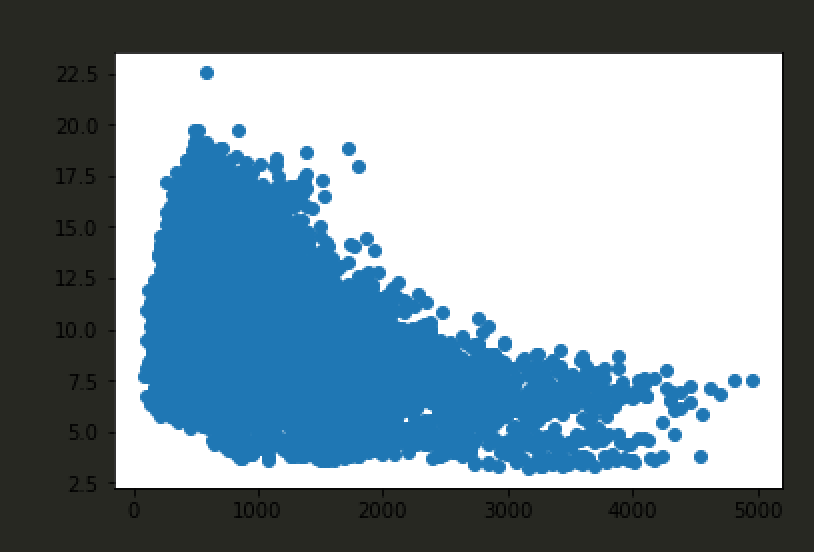
\includegraphics[scale=0.3]{Features/customers.png}
	\caption{Different Sales Customer ratio against number of customer}
\end{figure}

\begin{figure}[h]
	\centering
	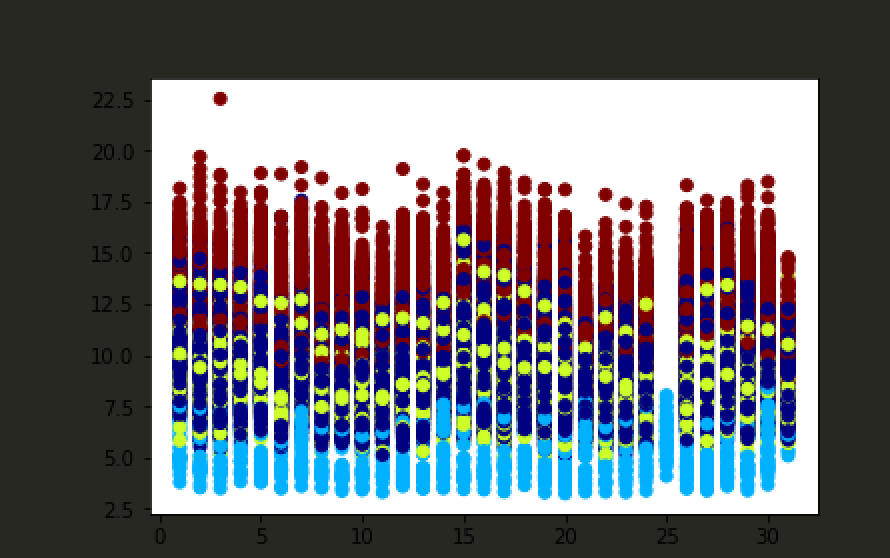
\includegraphics[scale=0.3]{Features/storetype.png}
	\caption{Different Sales Customer ratio against promotion state}
\end{figure}

From the above figure, we can see assortment, number of customers make a difference in sales customer ratio. In addition, store with promotion can aim a higher sales customer ratio, which demonstrates promotion state being a good feature to have. We also plotted the school and state holiday for reference, but the plots don't show much difference among holidays and working days.


 


\newpage

\section{Statement of team's work}

We $<A0148008J, A0141132B>$, as a team, certify that I have followed the CS3244 Machine Learning class guidelines for homework assignments.  In particular, I expressly vow that I have followed the Facebook rule in discussing with others in doing the assignment and did not take notes (digital or printed) from the discussions.  


\section{References}
\url{https://stackoverflow.com/questions/34178287/difference-between-objective-and-feval-in-xgboost}\\
\url{https://github.com/dmlc/xgboost/blob/master/demo/guide-python/custom_objective.py}\\
\url{http://blog.kaggle.com/2017/05/19/march-machine-learning-mania-1st-place-winners-interview-andrew-landgraf}\\


\end{document}